\chapter{Grouping and Evaluation}
\label{ch:grouping}

\section{The problem with implicit grouping}

Ordinary mathematical notation is compact because it leaves a great deal unsaid. The string $2 + 3 \times 4$ does not state which operation is to be performed first. A reader supplies the answer from a convention, according to which multiplication binds more tightly than addition, and obtains $14$ and not $20$. The convention is so thoroughly learned that it is rarely noticed, and yet it is part of the meaning of the expression. A reader who did not know it, or who applied a different one, would compute a different number from the same marks on the page.

Conventions of this kind multiply as notation grows. Subtraction and division associate to the left, so that $8 - 3 - 2$ is read as $(8-3)-2 = 3$ and not as $8-(3-2) = 7$. Exponentiation is conventionally read from the top down, so that $a^{b^c}$ means $a^{(b^c)}$ and not $(a^b)^c$. The two readings are not the same in general. With $a = 2$, $b = 3$, $c = 2$ the first gives $2^{9} = 512$ and the second gives $8^{2} = 64$. Programming languages add further layers, with tables of operator precedence that may run to a dozen levels, and with different languages making different choices about the same symbols.

There are two standard responses to this situation. One is to fully parenthesize, writing $2 + (3 \times 4)$ and $a^{(b^c)}$, so that nothing is left to convention. The other is to change the order of writing, as in the prefix notation $(\mathtt{+}\ 2\ (\mathtt{*}\ 3\ 4))$ used by Lisp-family languages, where the operator comes first and the grouping is carried entirely by brackets. Both responses make the structure of the expression explicit. Both also make it harder to read at a glance, because a bracket is a small mark that must be matched against a distant partner.

\section{Circles}

SpherePOP takes the second response and replaces the brackets by a visual boundary. An expression is drawn as a closed curve with the name of an operator written on it, and the operands of the operator are drawn inside. An operand may itself be a circle. A circle that encloses nothing but plain values, such as numbers, is the simplest kind of computation, and a circle that encloses other circles describes a computation whose inner parts must be completed before the outer one can be.

\begin{figure}[t]
\centering
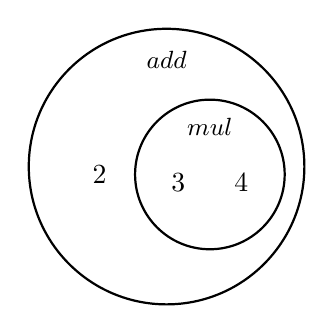
\begin{tikzpicture}
\draw[thick] (0,0) circle (1.75cm);
\node[font=\small] at (0,1.35) {$\op{add}$};
\node at (-0.85,-0.1) {$2$};
\draw[thick] (0.55,-0.1) circle (0.95cm);
\node[font=\small] at (0.55,0.5) {$\op{mul}$};
\node at (0.15,-0.2) {$3$};
\node at (0.95,-0.2) {$4$};
\end{tikzpicture}
\caption{The expression $2 + 3\times 4$ as nested circles. The inner circle labelled $\op{mul}$ encloses the operands $3$ and $4$, and is itself an operand of the outer circle labelled $\op{add}$.}
\label{fig:first-circle}
\end{figure}

Figure~\ref{fig:first-circle} shows $2 + 3 \times 4$ in this form. Nothing in the drawing refers to a precedence table. The multiplication is inside the addition because the drawing puts it there, and the drawing for $(2 + 3) \times 4$ would put the addition inside the multiplication. The two expressions are different pictures, and so the question of which one is meant never arises.

In running text a circle is written $\cir{o\; t_1 \cdots t_n}$, where $o$ is the operator and $t_1,\dots,t_n$ are the enclosed operands, each of which is a value or another circle. The expression of Figure~\ref{fig:first-circle} is written $\cir{\op{add}\; 2\; \cir{\op{mul}\; 3\; 4}}$. The angle brackets are a typographical stand-in for the drawn boundary and carry no meaning of their own beyond marking where a circle begins and ends.

\section{Popping}

A circle is a description of a computation, and it is carried out by popping. A circle may be popped when everything inside it is already a value. Popping replaces the entire circle by the value that its operator produces from the enclosed operands. For the circle of Figure~\ref{fig:first-circle} only the inner circle can be popped at first, since the outer circle encloses an operand that is not yet a value. Popping the inner circle replaces it by $12$, which leaves the circle $\cir{\op{add}\; 2\; 12}$, and popping that circle gives $14$. Written as a sequence,
\[
\cir{\op{add}\; 2\; \cir{\op{mul}\; 3\; 4}}
\;\longrightarrow\;
\cir{\op{add}\; 2\; 12}
\;\longrightarrow\;
14 .
\]
Each arrow is one pop, and each pop removes exactly one circle from the expression. These two facts, that a pop needs all operands to be values and that a pop removes exactly one circle, are the foundation of the results proved in Chapter~\ref{ch:order}.

Several circles may be ready at the same time. In $\cir{\op{add}\; \cir{\op{mul}\; 2\; 3}\; \cir{\op{mul}\; 4\; 5}}$ both multiplications can be popped, and the notation does not say which one comes first. The choice turns out to be irrelevant: whichever is popped first, the other is still ready afterward, and the final value is $26$ either way. Making this precise, and proving it, is the main business of Chapter~\ref{ch:order}.

\section{What the notation leaves out}

It is worth being explicit about what SpherePOP does not provide, because the omissions are deliberate. There are no precedence rules, since grouping is always drawn. There is no implicit conversion between kinds of value, since a circle either accepts the operands it is given or does not. There is no assignment, no loop, and no hidden state, since popping only replaces a circle by a value. And there is no fixed list of operators, since the notation does not care what an operator does, only that it takes some values in and gives a value back.

That last point is what makes the notation more than a curiosity of arithmetic. The operators in this book include the usual numerical ones, but also operators that rotate a picture, recolour it, and place two pictures side by side. The same circles, the same popping rule, and the same theorems apply to all of them. An expression such as $\cir{\op{rotate}\; \cir{\op{recolor}\; I\; \mathrm{red}}\; 90}$ is read exactly as the arithmetic expression above: the inner circle is popped first, yielding a picture, and the outer circle then rotates that picture. The distinction between numbers and pictures is handled by sorts, which are introduced in Chapter~\ref{ch:sorts}, and not by changing the evaluation rule.

A second kind of generality concerns what is allowed inside a circle. A circle may enclose a symbol, a name standing for a value that is not yet known. Such a circle cannot be popped, because its operator has nothing to compute with, and so it simply stays in the expression. This is how the notation keeps an expression such as $x^{2}$ unevaluated until $x$ is supplied, and it is the subject of Chapter~\ref{ch:symbols}.

\section{Reading a nested circle}

A useful habit is to read a nested expression from the inside out. The innermost circles, the ones that enclose no other circle, are the first candidates for popping. After they are replaced, a new set of innermost circles appears, and the process repeats. The number of times the process repeats is the greatest depth of nesting in the original expression, a quantity that reappears in Chapter~\ref{ch:order} as the number of rounds needed if all ready circles are popped simultaneously.

\begin{example}
Consider $\cir{\op{pow}\; \cir{\op{add}\; 1\; 1}\; \cir{\op{mul}\; 2\; \cir{\op{sub}\; 5\; 2}}}$. The innermost circles are $\cir{\op{add}\; 1\; 1}$ and $\cir{\op{sub}\; 5\; 2}$, and they pop to $2$ and $3$. The expression is now $\cir{\op{pow}\; 2\; \cir{\op{mul}\; 2\; 3}}$, whose only innermost circle pops to $6$, leaving $\cir{\op{pow}\; 2\; 6}$, which pops to $64$. The expression contains four circles, and four pops were needed. \hfill$\triangleright$
\end{example}

\section*{Exercises}

\begin{exercise}[\dag]\label{ex:ch1-write}
Write $2 + 3 \times 4$ and $(2+3)\times 4$ as circle expressions in the linear notation, and compute both values.
\end{exercise}

\begin{exercise}[\dag]\label{ex:ch1-tower}
Write the two groupings of $a^{b^c}$ as circle expressions using the operator $\op{pow}$. Compute both for $(a,b,c) = (2,3,2)$.
\end{exercise}

\begin{exercise}[\dag]\label{ex:ch1-pops}
Give every pop sequence for $\cir{\op{add}\; \cir{\op{mul}\; 2\; 3}\; \cir{\op{sub}\; 9\; 4}}$. How many are there, and do they reach the same value?
\end{exercise}

\begin{exercise}
Convert $((1+2)\times(3+4)) - 5$ to a circle expression, draw it as nested circles, and list the circles in an order in which they could be popped.
\end{exercise}

\begin{exercise}
Explain in a few sentences why the expression $8 - 3 - 2$ requires a convention in ordinary notation but has two distinct circle expressions. Write both.
\end{exercise}
